\section{Arranjos Produtivos Locais (APL) e sua relevância}

Arranjos Produtivos Locais (APL) são concentrações territoriais de empresas especializadas em determinado setor, articuladas com governos, associações, instituições de ensino, pesquisa e crédito \parencite{redeSist_guia, sebrae_apl}. Esses arranjos refletem vantagens comparativas locais e vêm sendo objeto de políticas públicas integradas que mobilizam infraestrutura, energia, transportes, comunicações, crédito e inovação \parencite{mdic_mapeamento_apl}. Entre essas dimensões, a formação profissional ocupa papel central, pois conecta diretamente a base produtiva regional com a qualificação da força de trabalho.

O fortalecimento dos APLs depende de transformar vantagens comparativas em ganhos efetivos de produtividade. Trabalhadores com formação em Educação Profissional e Tecnológica (EPT) executam as mesmas atividades de forma mais eficiente, adotam tecnologias e elevam a qualidade da produção, o que sustenta renda e competitividade regional \parencite{lastres_cassiolato}. Assim, o mapeamento dos APLs oferece aos estados não apenas uma justificativa para investimentos, mas sobretudo uma orientação clara sobre quais setores estratégicos devem guiar a expansão da EPT nos Planos de Aplicação do PROPAG.


\subsection{Setores destacados – Observatório EPT Fundação Itaú}

O Observatório EPT, desenvolvido pela Fundação Itaú Educação e Trabalho, 
disponibiliza uma ferramenta interativa para a identificação de setores produtivos 
destacados em cada estado e microrregião. O observatório está disponível neste link:  
\href{https://observatorioitau.org.br/}{Observatório da Fundação Itaú}\footnote{A equipe do Banco Mundial e da FGV responsável por este relatório não participou da produção 	deste aplicativo interativo. A presente referência é feita apenas para informar sobre 	uma ferramenta de apoio que pode ser utilizada por analistas na preparação dos 	Planos de Aplicação do PROPAG. Para informações adicionais sobre o Observatório EPT, 
recomenda-se contatar diretamente a Fundação Itaú.} A ferramenta utiliza dados da Relação Anual de Informações Sociais (RAIS), base  administrativa do Ministério do Trabalho que registra vínculos formais de emprego 
no Brasil. A partir dessas informações, o painel permite ordenar arranjos produtivos 
locais (APLs) pelo número de empregos, empresas e quocientes locacionais, 
indicando quais atividades concentram maior relevância econômica. A navegação é 
intuitiva: o usuário seleciona o estado, aplica filtros por setor econômico 
(classificação CNAE -- Classificação Nacional de Atividades Econômicas) ou por 
território, e obtém um retrato atualizado das áreas produtivas mais relevantes. Essas 
informações constituem um ponto de partida útil para relacionar a oferta de Educação 
Profissional e Tecnológica (EPT) com as necessidades do mercado de trabalho regional.

\textbf{Classificação CNAE 2.0}  
A base de organização dos setores no Observatório é a \emph{Classificação Nacional 
	de Atividades Econômicas} (CNAE 2.0), adotada oficialmente pelo IBGE e por todos 
os órgãos da administração pública.  A denominação “2.0” refere-se à segunda 
revisão da classificação, em vigor desde 2006, que atualizou a versão inicial dos 
anos 1990. A CNAE é hierárquica e possui cinco níveis: 
\underline{Seções}, que abrangem 21 grandes categorias designadas por letras de A a U 
(como Agricultura, Indústrias de Transformação, Educação, Saúde); 
\underline{Divisões}, identificadas por dois dígitos; 
\underline{Grupos}, com três dígitos; 
\underline{Classes}, de quatro dígitos; e 
\underline{Subclasses}, de sete dígitos, utilizadas para registros administrativos mais 
detalhados.  

No painel do Observatório, o ponto de entrada usual é o nível de \underline{Seção}. Por exemplo, 
a Seção A corresponde à \emph{Agricultura, Pecuária, Produção Florestal, Pesca e 
	Aquicultura}, que se relaciona diretamente com cursos técnicos em Agropecuária, 
Agroindústria e Recursos Naturais. A Seção I cobre \emph{Alojamento e Alimentação}, 
setor ligado a cursos de Hospedagem, Guia de Turismo e Gastronomia. Já a Seção F, 
\emph{Construção}, pode ser associada a formações em Edificações, Eletrotécnica e 
Segurança do Trabalho. A Tabela~\ref{tab:rais_cnae} apresenta a distribuição do emprego formal registrada na 
RAIS em 2023 e 2024 segundo a classificação por Seções da CNAE 2.0 no Brasil. 
Nas seções seguintes deste relatório será feita uma exploração adicional dessas 
informações, com vistas a apoiar o planejamento da expansão da Educação 
Profissional e Tecnológica (EPT).

\begin{table}[!htbp]
	\centering
	\caption{Empregos formais por Seção CNAE 2.0 (Brasil, RAIS 2023–2024)}
	\label{tab:rais_cnae}
	\footnotesize
	\setlength{\tabcolsep}{4pt}
	\begin{tabular}{@{\extracolsep{5pt}} p{1cm} p{7.7cm} r r}
		\textbf{Seção} & \textbf{Denominação oficial} & \textbf{2023} & \textbf{2024} \\
		\hline\\[-1.2ex]
		A & Agricultura, Pecuária, Produção Florestal, Pesca e Aquicultura & 1.786.999 & 1.799.906 \\
		B & Indústrias Extrativas & 271.027 & 281.975 \\
		C & Indústrias de Transformação & 7.830.162 & 8.124.440 \\
		D & Eletricidade e Gás & 135.379 & 138.909 \\
		E & Água, Esgoto, Atividades de Gestão de Resíduos e Descontaminação & 382.135 & 391.845 \\
		F & Construção & 2.849.438 & 2.960.420 \\
		G & Comércio; Reparação de Veículos Automotores e Motocicletas & 10.268.346 & 10.571.310 \\
		H & Transporte, Armazenagem e Correio & 2.696.919 & 2.821.899 \\
		I & Alojamento e Alimentação & 2.161.320 & 2.250.082 \\
		J & Informação e Comunicação & 1.196.117 & 1.233.464 \\
		K & Atividades Financeiras, de Seguros e Serviços Relacionados & 1.064.650 & 1.090.020 \\
		L & Atividades Imobiliárias & 197.167 & 200.719 \\
		M & Atividades Profissionais, Científicas e Técnicas & 1.550.526 & 1.633.457 \\
		N & Atividades Administrativas e Serviços Complementares & 5.789.290 & 6.170.237 \\
		O & Administração Pública, Defesa e Seguridade Social & 53.102 & 54.026 \\
		P & Educação & 1.900.395 & 1.958.241 \\
		Q & Saúde Humana e Serviços Sociais & 2.867.154 & 3.025.304 \\
		R & Artes, Cultura, Esporte e Recreação & 302.833 & 332.677 \\
		S & Outras Atividades de Serviços & 1.164.410 & 1.226.083 \\
		U & Organismos Internacionais e Outras Instituições Extraterritoriais & 4.432 & 4.468 \\
		\hline
		 & \textbf{Total} & \textbf{44.472.798} & \textbf{46.270.514} \\
		\hline\\[-1.6ex]
	\end{tabular}

\vspace{0.5em}
\begin{minipage}{0.9\textwidth}
	\footnotesize \textit{Fonte:} Ministério do Trabalho e Emprego (MTE), 
	Relação Anual de Informações Sociais (RAIS 2023 e 2024, dados parciais) 
	\href{https://www.gov.br/trabalho-e-emprego/pt-br/assuntos/estatisticas-trabalho/rais/rais-2024/rais-2024-parcial/apresentacao-rais-2024-parcial.pdf}{(link)}.
\end{minipage}
\end{table}


\textbf{Definição de APL}  
No Observatório, a identificação de um arranjo produtivo local parte da contagem 
de empregos formais por setor (CNAE) e território na RAIS. Para medir a 
especialização relativa, utiliza-se o \emph{quociente locacional} (QL), calculado como:  

\[
QL_{i,r} = \frac{\tfrac{E_{i,r}}{E_{r}}}{\tfrac{E_{i,B}}{E_{B}}}
\]

em que \(E_{i,r}\) é o emprego formal do setor \(i\) na região \(r\); \(E_{r}\) é o emprego total 
da região; \(E_{i,B}\) é o emprego do setor \(i\) na área de referência (Brasil ou unidade 
federativa); e \(E_{B}\) é o emprego total da área de referência.\footnote{IBGE/CONCLA 
	– Comissão Nacional de Classificação. \emph{CNAE 2.0: Estrutura e Notas 
		Explicativas}, 2006. Disponível em: \url{https://concla.ibge.gov.br/}}  

Valores de \(QL > 1\) indicam que o setor é relativamente mais concentrado na região 
do que na média nacional ou estadual, sugerindo a presença de uma especialização 
produtiva. A partir desse critério, aliado a limites mínimos de número de empresas ou 
empregos, são listados os setores e territórios como potenciais APLs.

\begin{figure}[!htbp]
	\centering
	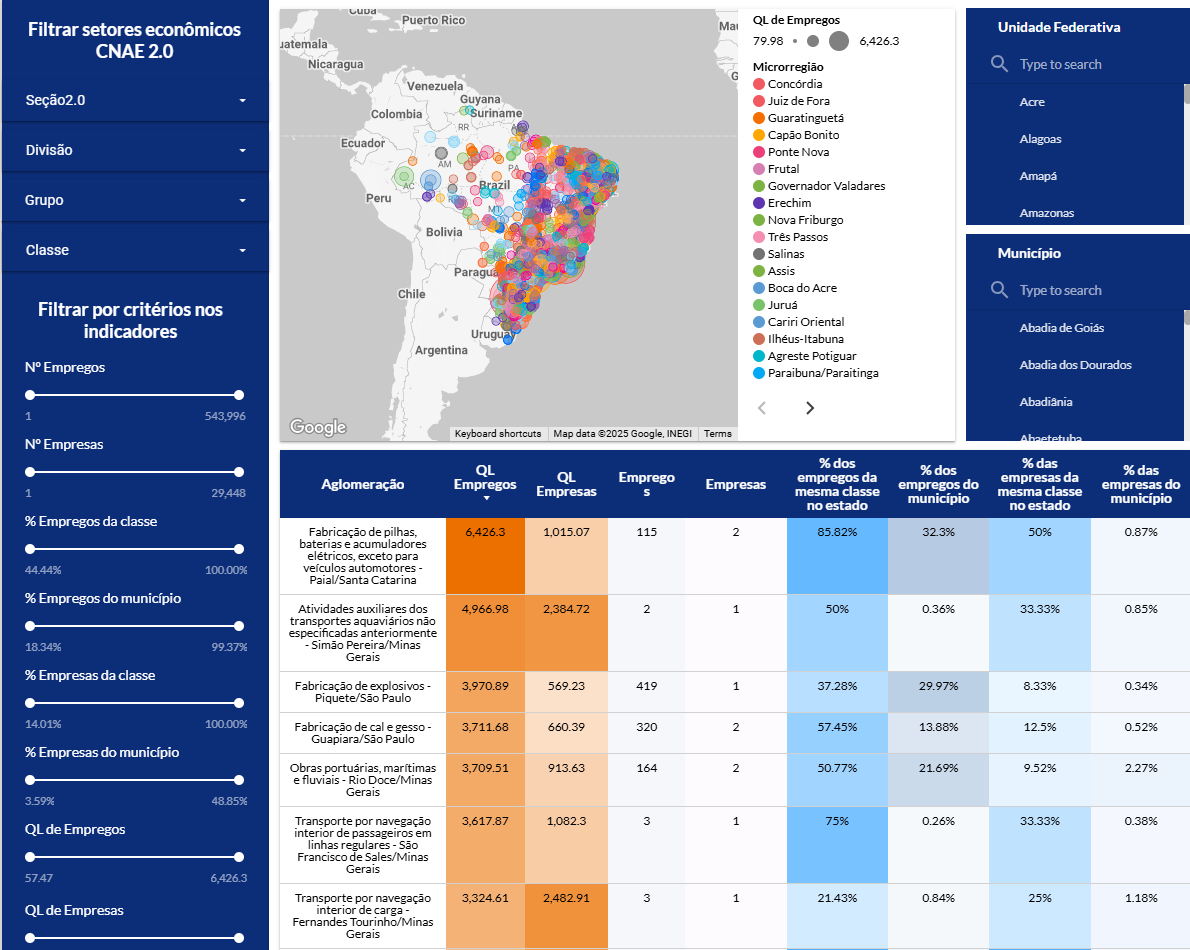
\includegraphics[width=0.9\textwidth]{images/2d_ObsEPTITAU.png}
	\caption{Painel interativo do Observatório EPT Fundação Itaú, 
		com filtros por CNAE, mapa de distribuição e tabela de aglomerações produtivas locais.}
	\label{fig:obs_ept}
\end{figure}

\textbf{Elementos do painel interativo}  
O Observatório EPT apresenta a informação por meio de um painel em ambiente 
Looker Studio, composto por quatro partes principais que funcionam de forma 
integrada: filtros, mapa, tabela e seleção territorial.  

\textbf{Filtros principais.} Localizados no lado esquerdo, permitem refinar a análise 
por \underline{CNAE 2.0} em diferentes níveis (Seção, Divisão, Grupo ou Classe) e 
aplicar controles deslizantes (\emph{sliders}) para limitar o número mínimo de empregos, 
de empresas ou o valor do quociente locacional. Esses filtros ajudam o usuário a 
focar em setores e atividades com maior peso relativo em uma região.  

\textbf{Mapa.} A parte superior do painel mostra a distribuição geográfica dos setores 
selecionados, por município ou microrregião. A cor dos polígonos representa a 
intensidade do indicador (empregos, empresas ou QL), permitindo visualizar 
rapidamente os pontos de maior concentração.  

\textbf{Tabela.} A parte inferior apresenta a lista detalhada das aglomerações 
produtivas locais (setor + território), que pode ser ordenada pelo usuário. Entre as 
colunas estão: número de empregos, número de empresas, quociente locacional 
para empregos e para empresas, além da participação percentual do setor no 
município e no estado.  

\textbf{Seleção territorial.} No lado direito, há menus suspensos que permitem escolher 
a unidade da federação (UF) ou o município de interesse. A escolha atualiza o mapa 
e a tabela de forma automática, facilitando o recorte espacial.  

Esses elementos, usados em conjunto, permitem ao analista explorar de forma 
interativa quais setores produtivos apresentam maior concentração regional, onde 
estão localizados e como se comparam em termos de emprego e empresas.


\subsection{Arranjos Produtivos Locais Ocupacionais (APLO)}

Apresentamos uma abordagem baseada em ocupações (CBO) para a identificação de arranjos produtivos locais, utilizando microdados da RAIS para os anos de 2023 e 2024. A metodologia estima a especialização relativa de ocupações nos níveis municipal, regional e estadual. Por se apoiar diretamente na estrutura ocupacional, esta abordagem permite associar os arranjos identificados aos cursos técnicos do Catálogo Nacional de Cursos Técnicos (CNCT), oferecendo subsídios para o planejamento da oferta de EPT alinhada ao perfil produtivo dos territórios.

\textbf{Identificação de Ocupações com Especialização Local}

A identificação das ocupações com possível base produtiva local é realizada a partir da base RAIS, utilizando códigos CBO de 4 dígitos (famílias ocupacionais) e aplicando a métrica de quociente locacional (QL), também conhecida como \textit{Revealed Comparative Advantage} (RCA). O QL compara a participação de uma ocupação no total de vínculos formais do município com a respectiva participação da mesma ocupação no total de vínculos do Brasil:

\[
QL_{m,o} = \frac{\frac{E_{m,o}}{E_m}}{\frac{E_{br,o}}{E_{br}}}
\]

Onde:

\begin{itemize}
	\item $E_{m,o}$ = número de vínculos para ocupação $o$ no município $m$
	\item $E_m$ = total de vínculos no município $m$
	\item $E_{br,o}$ = vínculos para ocupação $o$ no Brasil
	\item $E_{br}$ = total de vínculos no Brasil
\end{itemize}

Considera-se que um município tem especialização local em determinada ocupação se $QL_{m,o} \geq 1$, desde que haja também um mínimo de 30 vínculos registrados para aquela ocupação no município. A análise é aplicada para os anos de 2023 e 2024 e, como critério adicional de robustez, considera-se apenas os casos em que a ocupação satisfaz os critérios em ambos os anos (persistência).

\vspace{1em}

\textbf{Métricas de Diversidade, Ubiquidade e Complexidade}

A partir da matriz binária de presença de ocupações com especialização local ($QL_{m,o} \geq 1$), são extraídas medidas de estrutura da base produtiva local. Essas métricas complementam a identificação de APLs e ajudam a caracterizar os territórios e as ocupações:

\begin{itemize}
	\item \underline{Diversidade municipal}: mede a variedade de especializações ocupacionais observadas em cada município. Utilizamos duas métricas:
	\begin{itemize}
		\item \textit{Índice de Herfindahl-Hirschman (HHI)} — indica concentração; valores altos sugerem baixa diversidade.
		\item \textit{Entropia de Shannon} — mede dispersão; valores altos indicam maior diversidade.
	\end{itemize}
	
	\[
	HHI_m = \sum_o \left(\frac{E_{m,o}}{E_m}\right)^2
	\qquad\text{e}\qquad
	Shannon_m = -\sum_o \left(\frac{E_{m,o}}{E_m} \cdot \log \left( \frac{E_{m,o}}{E_m} \right) \right)
	\]
	
	\item \underline{Ubiquidade ocupacional}: número de municípios nos quais a ocupação apresenta especialização ($QL \geq 1$).
	
	\item \underline{Complexidade ocupacional}: média da diversidade (HHI ou Shannon) dos municípios onde a ocupação aparece com $QL \geq 1$.
	
	\item \underline{Complexidade municipal}: média da ubiquidade das ocupações especializadas naquele município.
\end{itemize}

\textbf{Correspondência das Ocupações (CBO) com Cursos Técnicos (CNCT)}

Para cada ocupação com especialização local identificada no passo anterior, realiza-se uma correspondência com cursos técnicos do Catálogo Nacional de Cursos Técnicos (CNCT), utilizando métodos de similaridade semântica entre descrições de cursos e ocupações.
 A correspondência é baseada em embeddings gerados a partir de modelos de linguagem e envolve múltiplos critérios (semântica, TF-IDF, vetores densos), resultando em uma pontuação final de similaridade ($\text{final\_score}$). Para cada ocupação (CBO de 6 dígitos), são selecionados os 20 cursos mais próximos. Em seguida, agregamos esses resultados para o nível de família ocupacional (CBO de 4 dígitos), retendo os 5 cursos com maior pontuação média. Essa etapa produz, para cada ocupação com RCA ≥ 1, uma lista dos cursos técnicos mais coerentes com seu perfil, permitindo inferir quais formações técnicas seriam mais adequadas ao perfil produtivo local.


\textbf{Correspondência das Ocupações (CBO) com Cursos Técnicos (CNCT)}

Para cada ocupação com especialização local identificada no passo anterior, realiza-se uma correspondência com cursos técnicos do Catálogo Nacional de Cursos Técnicos (CNCT), utilizando métodos de similaridade semântica entre descrições de cursos e ocupações.
A correspondência é baseada em embeddings gerados a partir de modelos de linguagem e envolve múltiplos critérios (semântica, TF-IDF, vetores densos), resultando em uma pontuação final de similaridade ($\text{final\_score}$). Para cada ocupação (CBO de 6 dígitos), são selecionados os 20 cursos mais próximos. Em seguida, agregamos esses resultados para o nível de família ocupacional (CBO de 4 dígitos), retendo os 5 cursos com maior pontuação média.
Essa etapa produz, para cada ocupação com RCA ≥ 1, uma lista dos cursos técnicos mais coerentes com seu perfil, permitindo inferir quais formações técnicas seriam mais adequadas ao perfil produtivo local.


\textbf{Integração com Dados de Matrícula do Censo Escolar}

Os cursos técnicos identificados como relevantes para os APLs são cruzados com os dados de matrícula disponíveis no Censo Escolar de 2023 e 2024. A comparação é realizada por estado (UF) e, quando possível, desagregada por curso e por dependência administrativa da escola (rede federal, estadual, municipal ou privada). Essa integração permite evidenciar eventuais lacunas entre a demanda ocupacional (inferida a partir dos APLs) e a oferta educacional atual. Embora a correspondência entre denominações de cursos possa não ser exata, utilizamos normalizações de texto para aproximar os nomes de cursos técnicos do CNCT com os registrados no Censo.
